\documentclass[a4paper,11pt]{article}

% Packages
\usepackage{listings}
\lstset{
    breaklines=true, % Break long lines
    language=SQL, % Set language for syntax highlighting
    basicstyle=\small, % Set the font size
    numbers=none, % No line numbers
    frame=single % Add a frame around the code
}
\usepackage{placeins}
\usepackage{float}
\usepackage{caption}
\usepackage[utf8]{inputenc}
\usepackage{amsmath}
\usepackage{graphicx}
\usepackage{geometry}
\usepackage{enumitem}
\geometry{a4paper, margin=1in}

% Title and Author
\title{Project 3}
\author{Ahmed Tlili, Leon Petrinos, Mathilde Peruzzo}
\date{\today}

\begin{document}

\maketitle

\section*{Relational Schema}
\begin{itemize}
    \item \textbf{Store}(\underline{s\_id}, s\_address, phone\_number, manager\_id UNIQUE NOT NULL)\\
        FOREIGN KEY(manager\_id) REFERENCES Employee(employee\_id)
    \item \textbf{Employee}(\underline{e\_id}, e\_name, s\_id)\\
        FOREIGN KEY(s\_id) REFERENCES Store(s\_id)
    \item \textbf{Manufacturer}(\underline{m\_id}, m\_name)
    \item \textbf{Product}(\underline{p\_id}, p\_name NOT NULL, unit\_price NOT NULL, description,\\ discount\_percentage, m\_id NOT NULL)\\
        FOREIGN KEY(m\_id) REFERENCES Manufacturer(m\_id)
    \item \textbf{Paint}(\underline{p\_id}, base, color)\\
        FOREIGN KEY(p\_id) REFERENCES Product(p\_id)
    \item \textbf{Tool}(\underline{p\_id}, type)
    \item \textbf{Has\_in\_stock}(\underline{p\_id}, \underline{s\_id}, quantity NOT NULL )\\
        FOREIGN KEY(p\_id) REFERENCES Product(p\_id)\\
        FOREIGN KEY(s\_id) REFERENCES Store(s\_id)
    \item \textbf{Customer}(\underline{email}, c\_name, c\_address NOT NULL)\\
        PRIMARY KEY(email)
    \item \textbf{Purchase}(\underline{p\_id}, amount NOT NULL, p\_date NOT NULL, p\_time NOT NULL)
    \item \textbf{Contains\_purchase}(\underline{p\_id}, \underline{product\_id}, quantity NOT NULL)\\
        FOREIGN KEY(p\_id) REFERENCES Purchase(p\_id)\\
        FOREIGN KEY(product\_id) REFERENCES Product(p\_id)
    \item \textbf{Instore}(\underline{p\_id}, \underline{e\_id})\\
        FOREIGN KEY(p\_id) REFERENCES Purchase(p\_id)\\
        FOREIGN KEY(e\_id) REFERENCES Employee(e\_id)
    \item \textbf{Online}(\underline{p\_id}, rating, delivery\_fee NOT NULL, email NOT NULL)\\
        FOREIGN KEY(p\_id) REFERENCES Purchase(p\_id)\\
        FOREIGN KEY(email) REFERENCES Customer(email)
\end{itemize}

\section*{Stored Procedure}

\begin{enumerate}[label=(\alph*)]
    \item This stored procedure increases the discount of products that have never been sold by 10\% until the maximum discount is reached. Maximum discount is the input argument.
    If the current discount is already greater or equal to the maximum discount, the discount will not be increased.
    If when increasing the current discount, the maximum discount is reached surpassed, the discount will be set to the maximum discount (no more).
    Otherwise, the current discount will be increased by 10\%.
    \item
    \begin{lstlisting}
    CREATE OR REPLACE PROCEDURE DiscountInactiveProducts(IN max_discount INT)
    BEGIN
        DECLARE done INT DEFAULT 0;
        DECLARE current_pid INT;
        DECLARE current_discount INT;
    
        DECLARE product_cursor CURSOR FOR
            SELECT p_id, COALESCE(discount_pourcentage, 0)
            FROM Product
            WHERE COALESCE(discount_pourcentage, 0) < max_discount;
    
        DECLARE CONTINUE HANDLER FOR NOT FOUND SET done = 1;
    
        OPEN product_cursor;
    
        FETCH product_cursor INTO current_pid, current_discount;
    
        WHILE done = 0 DO

            IF (NOT EXISTS (
                SELECT 1
                FROM Contains_purchase
                WHERE product_id = current_pid)
            )
            THEN
                IF (current_discount + 10 > max_discount) THEN
                    SET current_discount = max_discount;
                ELSE 
                    SET current_discount = current_discount + 10;
                END IF;
    
                UPDATE Product
                SET discount_pourcentage = current_discount
                WHERE p_id = current_pid;
            END IF;
    
            FETCH product_cursor INTO current_pid, current_discount;
    
        END WHILE;
    
        CLOSE product_cursor;
    END
    \end{lstlisting}
    \item 
\end{enumerate}
Calling the procedure with maximum discount of 25\%\\
\includegraphics*[width=\textwidth]{images/call_to_procedure.png}
First 25 products (id and discount) before calling procedure:\\
\includegraphics*[width=\textwidth]{images/products_before.png}
First 25 products (id and discount) after calling procedure. Note that the products with id 1 to 20 have purchases, so only the discounts from 21 to 25 change. \\
\includegraphics*[width=\textwidth]{images/products_after.png}

\section*{Application Program}
The application handles all the errors gracefully.\\
This is the current menu of the application.\\
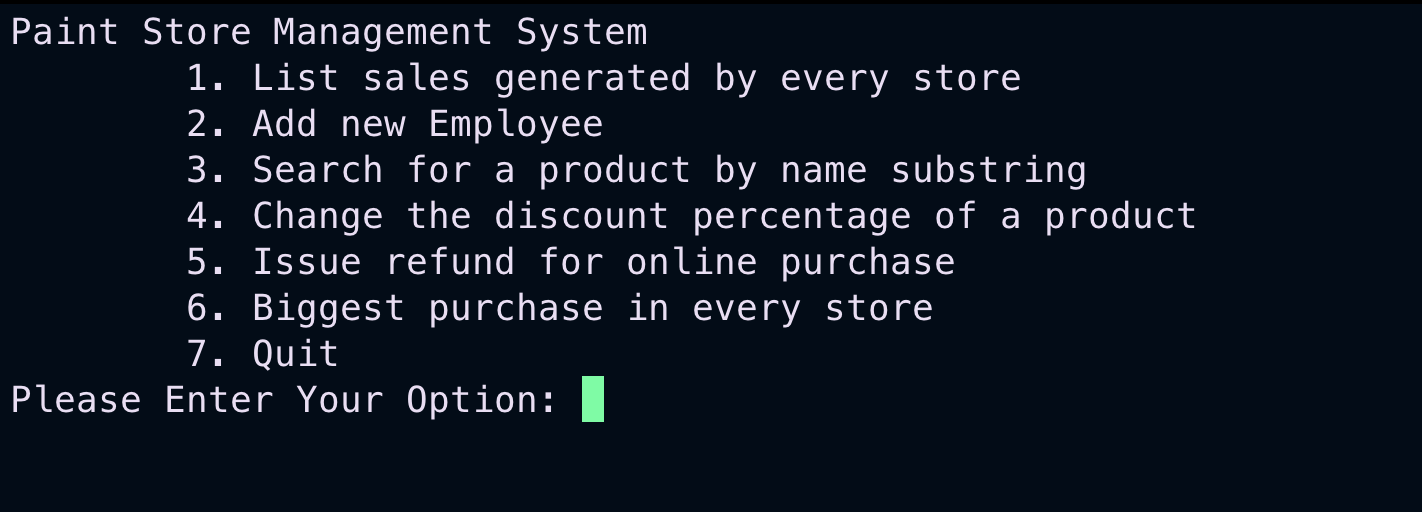
\includegraphics[width=0.9\textwidth]{images/menu.png}

\noindent
Let's discuss what each option does:
\begin{enumerate}[label=-]
    \item Type 1 to select Option 1: list sales generated by every store\\
        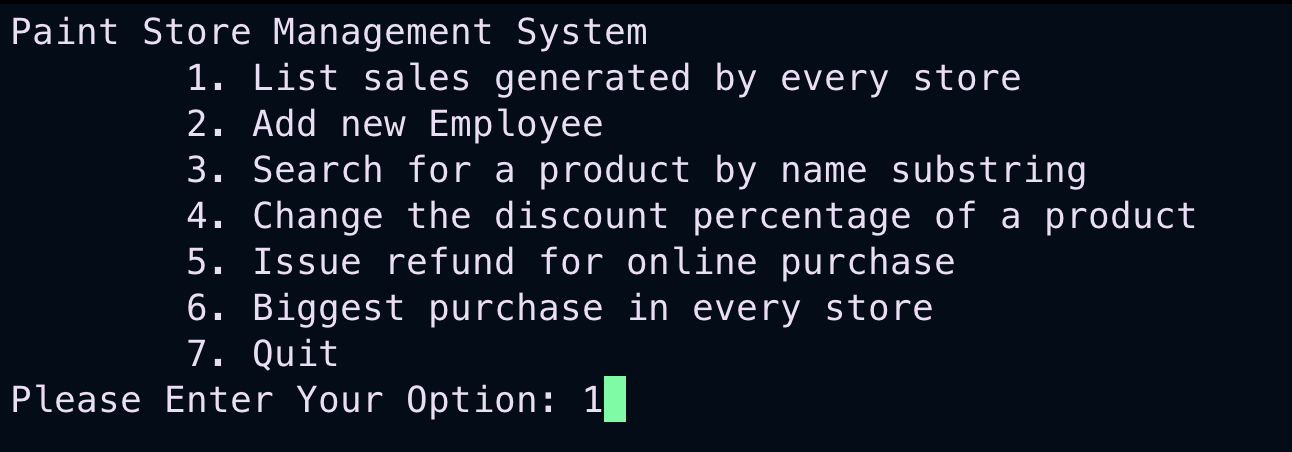
\includegraphics[width=0.9\textwidth]{images/menu_option_1_1.png}\\
        Output is the following:\\
        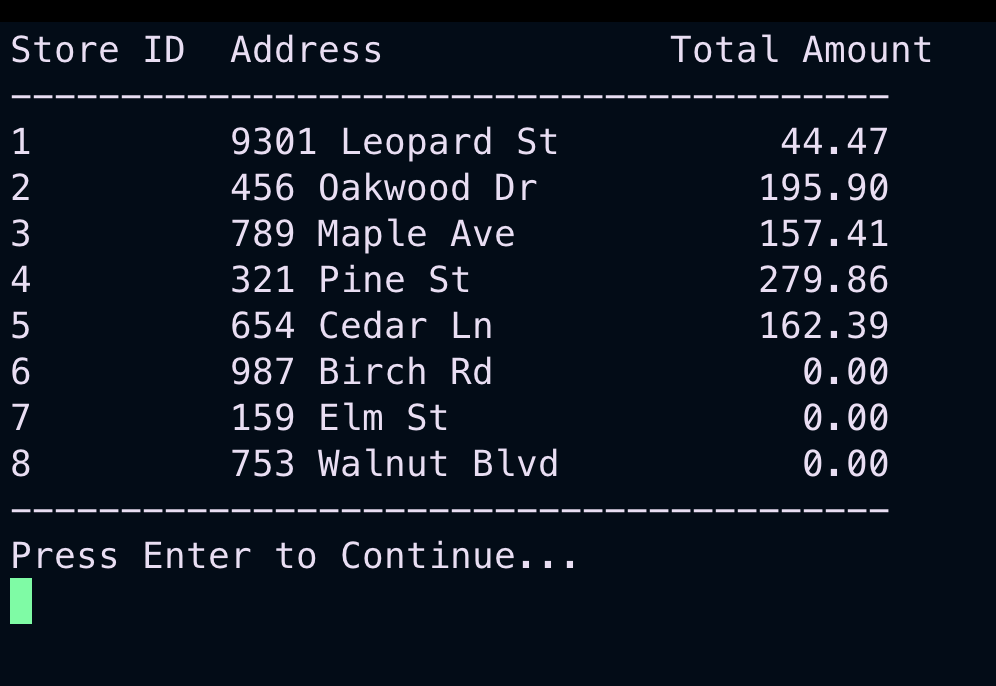
\includegraphics[width=0.9\textwidth]{images/menu_option_1_2.png}
    \item Type 2 to select Option 2: Add new Employee\\
        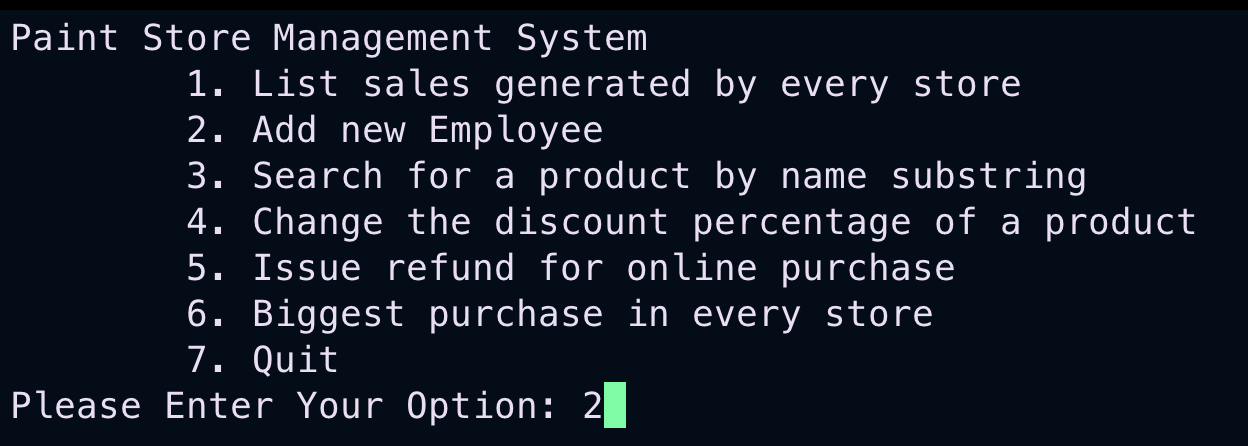
\includegraphics[width=0.9\textwidth]{images/menu_option_2_1.png}\\
        Just enter the name of the employee and the store he will be working
        for, output is the following:\\
        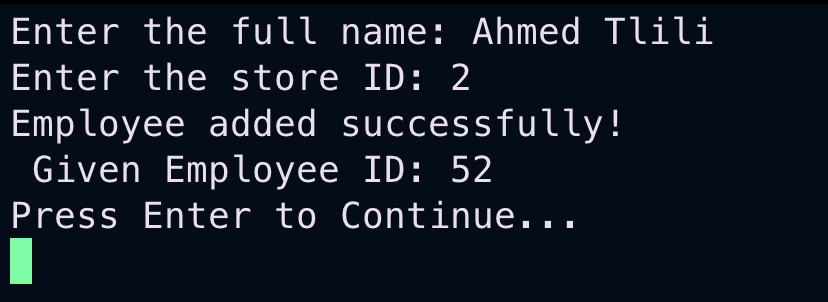
\includegraphics[width=0.9\textwidth]{images/menu_option_2_2.png}
    \item Type 3 to select Option 3: Search for a product by name substring\\
        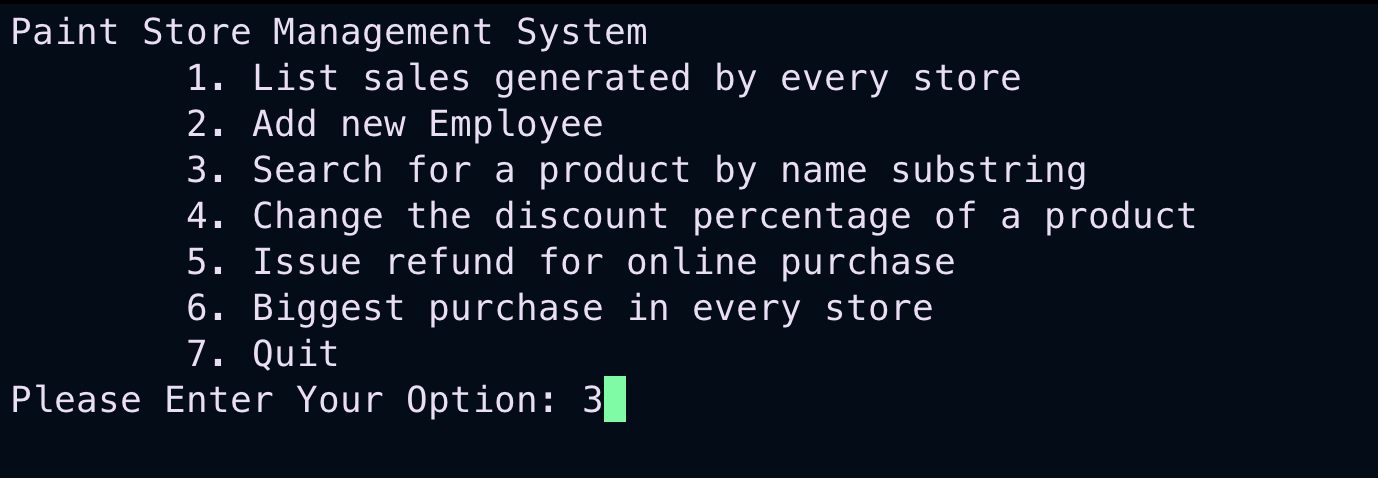
\includegraphics[width=0.9\textwidth]{images/menu_option_3_1.png}\\
        Example below shows the output when searching for the products with
        name containing "Peach"\\
        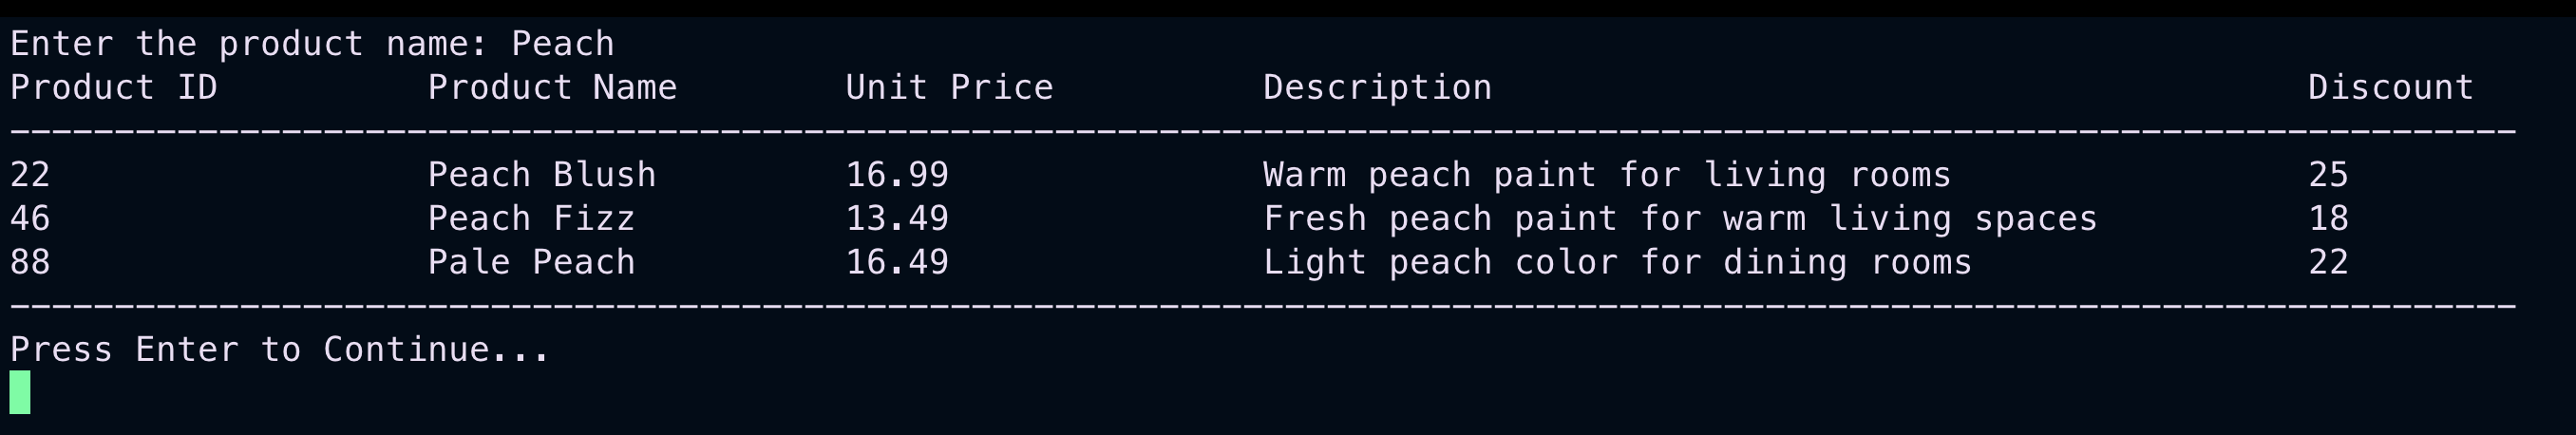
\includegraphics[width=0.9\textwidth]{images/menu_option_3_2.png}
    \item Type 4 to select Option 4: Change the discount percentatge of a product\\
        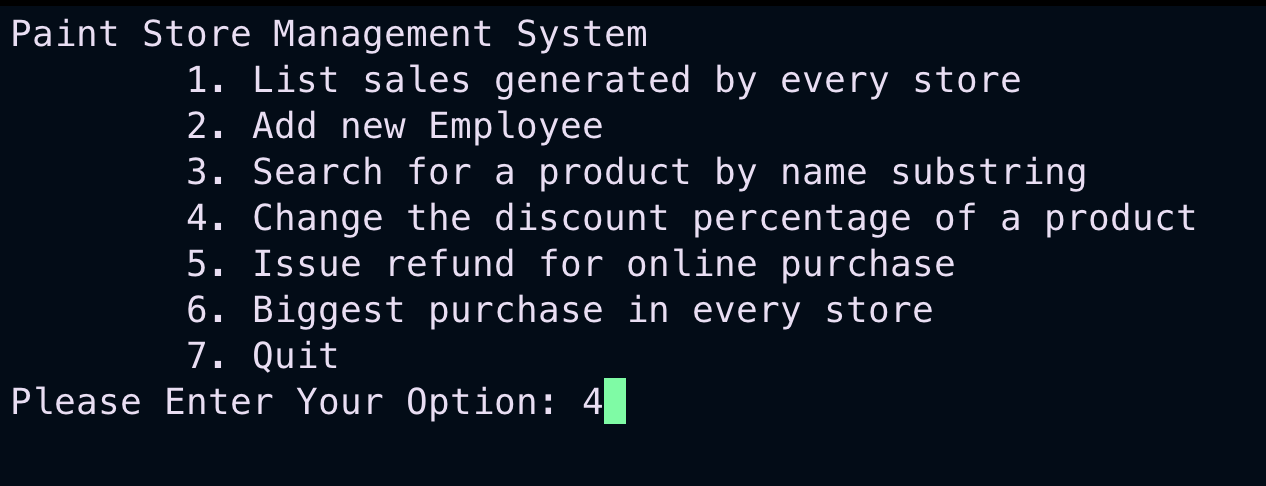
\includegraphics[width=0.9\textwidth]{images/menu_option_4_1.png}\\
        Just enter the ID of the product and the new discount percentage,
        output is the following:\\
        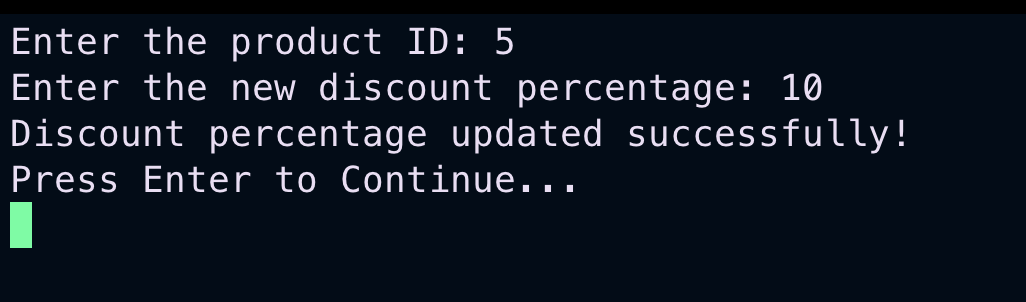
\includegraphics[width=0.9\textwidth]{images/menu_option_4_2.png}
    \item Type 5 to select Option 5: Issue refund for online purchase\\
        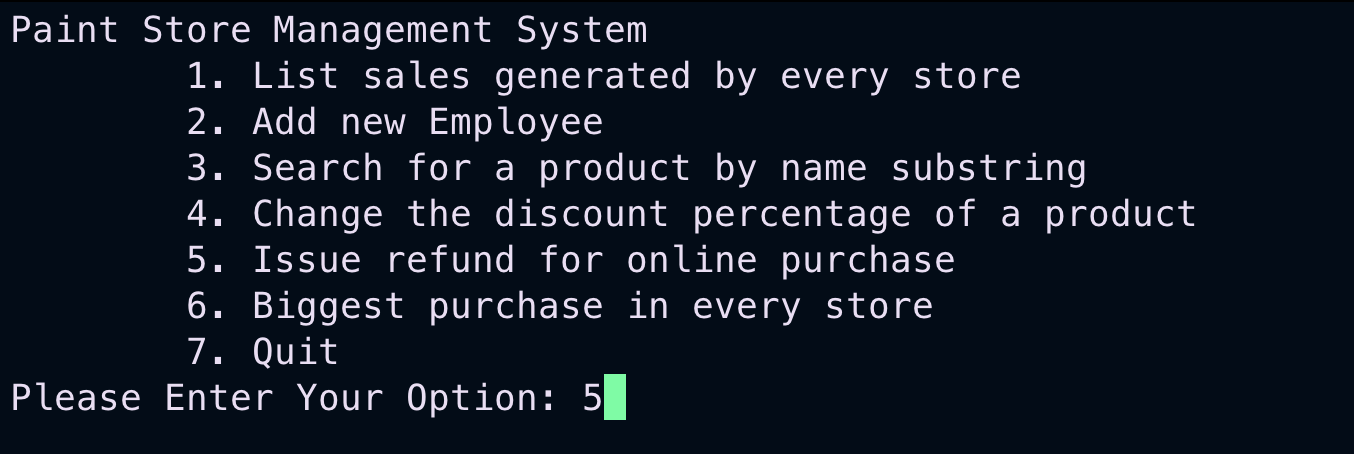
\includegraphics[width=0.9\textwidth]{images/menu_option_5_1.png}\\
        Just enter the email of the customer, a list of all his online purchases
        will be displayed, then you can select the purchase you want to refund
        by typing the correct number in the submenu. Output is the following:\\
        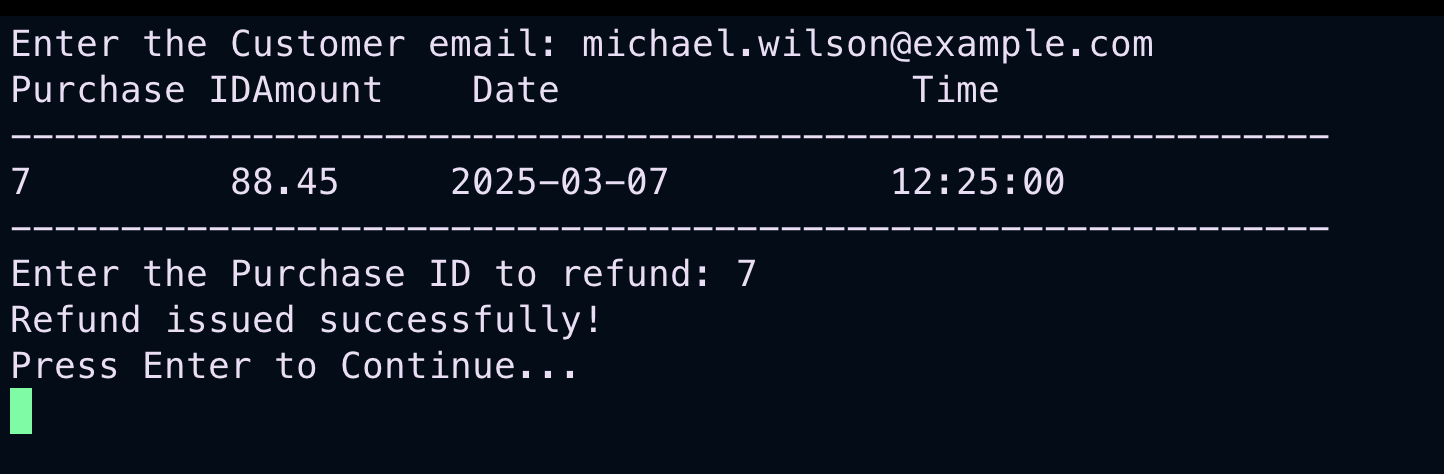
\includegraphics[width=0.9\textwidth]{images/menu_option_5_2.png}
    \item Type 6 to select Option 6: Biggest purchase in every store\\
        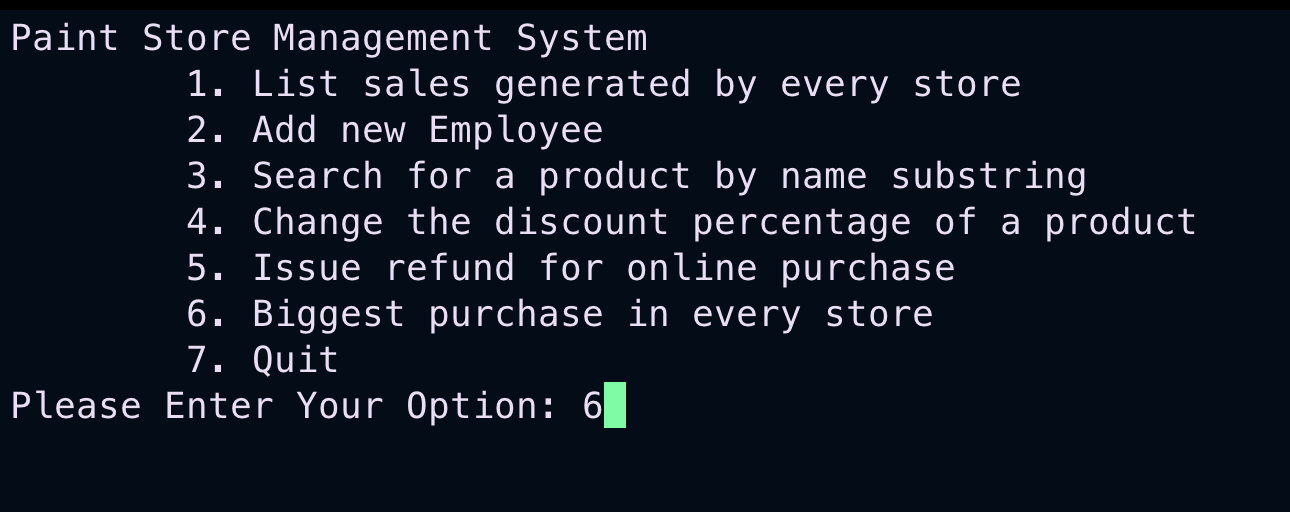
\includegraphics[width=0.9\textwidth]{images/menu_option_6_1.png}\\
        Output is the following:\\
        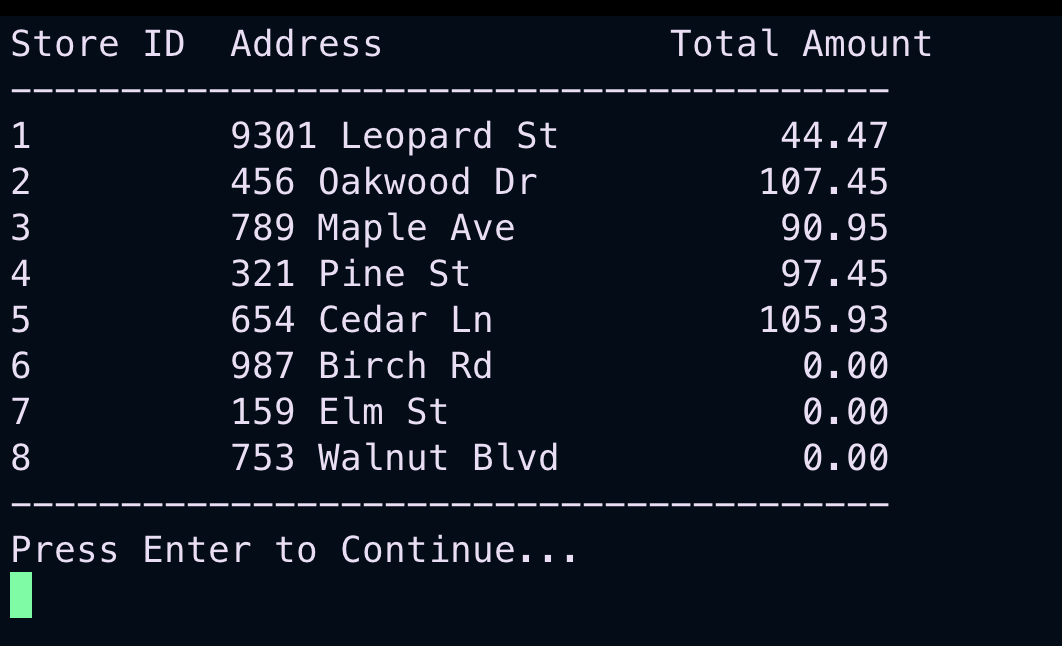
\includegraphics[width=0.9\textwidth]{images/menu_option_6_2.png}
    \item Type 7 to select Option 7: Quit\\
        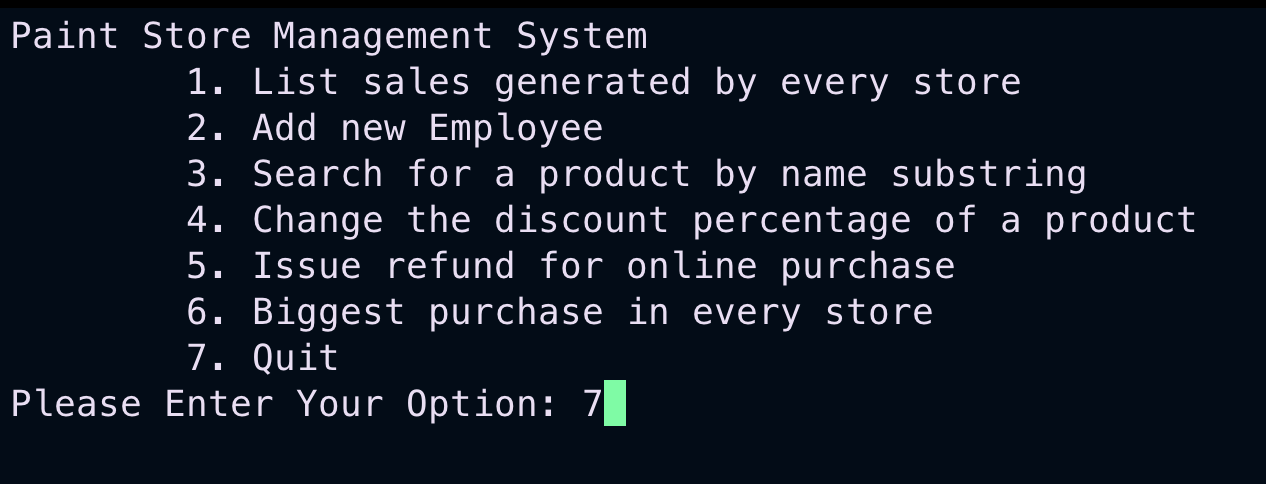
\includegraphics[width=0.9\textwidth]{images/menu_option_7_1.png}\\
        Correctly exits the application.\\
        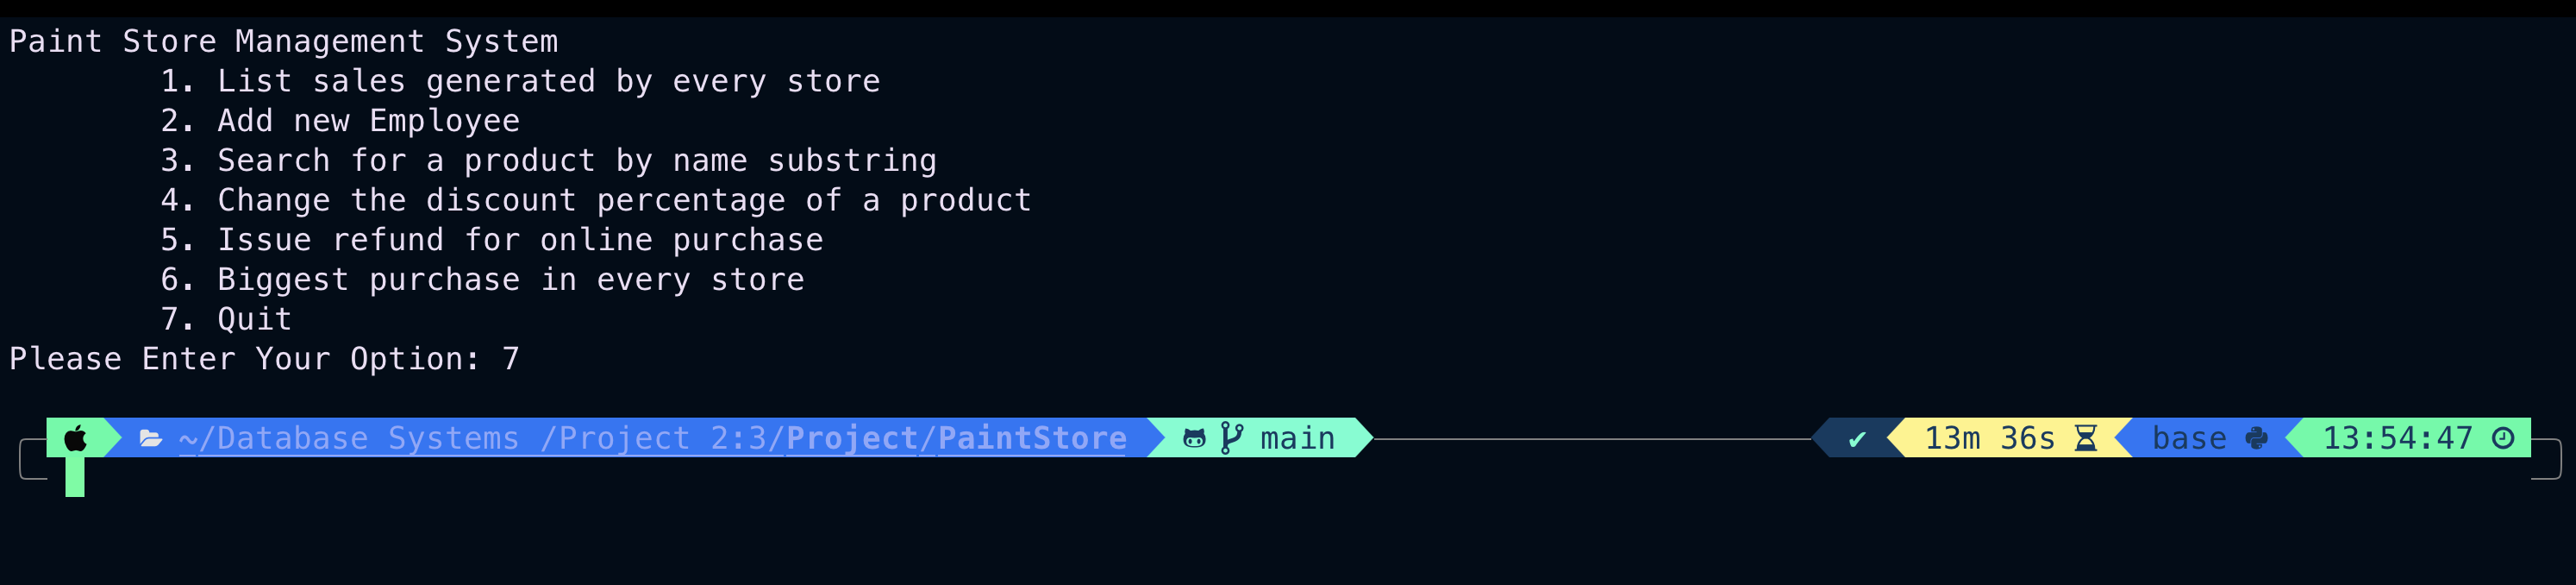
\includegraphics[width=0.9\textwidth]{images/menu_option_7_2.png}
\end{enumerate}

\section*{Indexing}

\subsection*{Index 1}

\begin{enumerate}[label=(\alph*)]
    \item 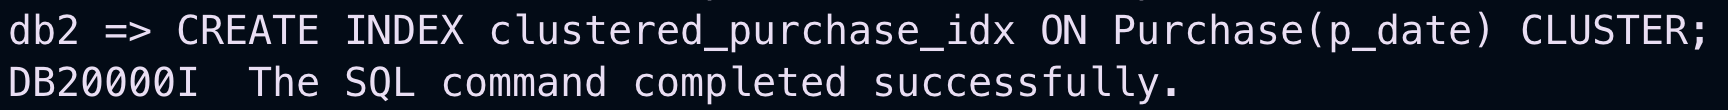
\includegraphics[width=0.9\textwidth]{images/idx1.png}
    \item A clustered index on purchase date in the Purchase table is beneficial because purchases are frequently analyed based on dates and date ranges.
    Thus, sorting the purchases by date allows for efficient range queries, making it faster to access data for accounting purposes.
    An example query that would benefit from this index is the following:
    \begin{lstlisting}
        SELECT SUM(amount) AS total
        FROM Purchase
        WHERE p_date >= '01/01/2025' AND p_date <= '12/31/2025';
    \end{lstlisting}
    This above query computes the total revenue for the year 2025. With this clustered index, the database can quickly locate the first matching row, and perform a sequential scan to retrieve all rows within the specified date range, without needing to follow the pointers of other data entries (value + rid), as in a non-clustered index, which could often leed to more IO.
\end{enumerate}

\subsection*{Index 2}
\begin{enumerate}[label=(\alph*)]
    \item 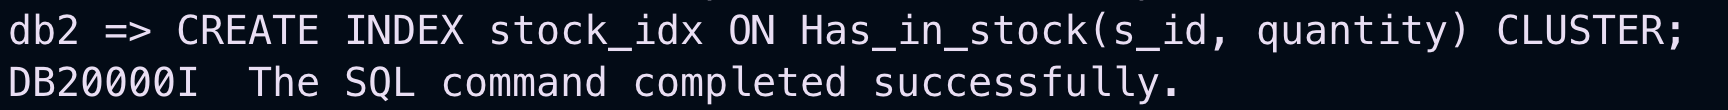
\includegraphics[width=0.9\textwidth]{images/idx2.png}
    \item This index is on the s\_id and quantity attribute of the Has\_in\_stock table.
    It is useful for this application to efficiently identify products that are running low in stock in a specific store, which is crucial for inventory management.
    An example query that would benefit from this index is the following:
    \begin{lstlisting}
        SELECT p_id
        FROM Has_in_stock
        WHERE s_id = 0 AND quantity < 5;
    \end{lstlisting}
    This query identifies all products of a particular store where the quantity of the product is very limited.
    The fact that it is a clustered index, again, allows for efficient range queries, making it faster to access data for inventory management purposes.
    It also makes sense to use a clustered index because the other attributes of the table are id's, which are certainly not needed in a sorted order.
\end{enumerate}
\section*{Visualisation}

\subsection*{Vis 1}

\subsection*{Vis 2}

\section*{Creativity}

\section*{Work Division}
We had two meetings to discuss the project and the work division. We decided to divide the work as follows:
\begin{itemize}
    \item Ahmed Tlili: Question 4 coding the application program
    \item Leon Petrinos: Question 3, 5 about indexing and stored procedures
    \item Mathilde Peruzzo: Question 6, 7 about visualisation and creativity
\end{itemize}


\end{document}

